\documentclass[12pt]{article}

% Packages
\usepackage{amsmath}
\usepackage[margin = 0.75 in]{geometry}
\usepackage[shortlabels]{enumitem}
\usepackage{tikz}

% Configuration
\title{15.3.27. (pg. 1068)}
\author{Arnav Patri}

% Notation
\renewcommand{\d}{\text{d}}

\begin{document}
	\maketitle
	\thispagestyle{empty}
	\[f(x, y) = x\]
	\[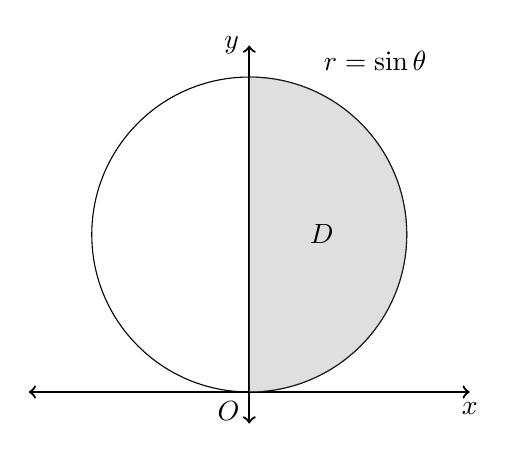
\begin{tikzpicture}[scale = 4]
		\draw[<->, thick] (-0.7, 0) -- (0.7, 0) node[below]{$x$};
		\draw[<->, thick] (0, -0.1) -- (0, 1.1) node[left]{$y$};
			\node[anchor = north east] at (0, 0) {$O$};
		\draw[radius = 0.5] (0, 0.5) circle;
		\draw[fill = lightgray, opacity = 0.5] (0, 0.5) -- (-90:0) arc(-90:90:0.5) -- cycle;
			\node at (0.23, 0.5) {$D$};
			\node at (0.4, 1.05){$r = \sin\theta$};
	\end{tikzpicture}\]
	\begin{enumerate}[(a)]
		\item
			Set up an iterated integral in polar coordinates for the volume of the solid under the graph of the given function and above the region $D$.
				\begin{align*}	
					\iint\limits_D f(x, y)\,\d A &= \int_0^{\frac{\pi}{2}}\int_0^{\sin\theta} f(r\cos\theta, r\sin\theta)r\,\d r\,\d\theta \\
						&= \int_0^{\frac{\pi}{2}}\int_0^{\sin\theta} r^2\cos\theta\,\d r\,\d\theta
				\end{align*}
		\item
			Evaluate the iterated integral to find the volume of the solid.
				\begin{align*}
					\int_0^{\frac{\pi}{2}}\int_0^{\sin\theta} r^2\cos\theta\,\d r\,\d\theta 
							&= \int_0^{\frac{\pi}{2}}\left[\frac{r^3\cos\theta}{3}\right]_0^{\sin\theta}\d\theta \\
						&= \int_0^{\frac{\pi}{2}}\left[\frac{\sin^3\theta\cos\theta}{3}\right]\d\theta \\
					u &= \sin\theta \qquad 
							\theta_1 = \sin(0) = 0 \qquad 
							\theta_2 = \sin\left(\frac{\pi}{2}\right) = 1 \\
					\d u &= \cos\theta\,\d\theta\\
					\int_0^{\frac{\pi}{2}}\left[\frac{\sin^3\theta\cos\theta}{3}\right]\d\theta
							&= \int_0^1\left[\frac{u^3}{3}\right]\d u \\
							&= \left[\frac{u^4}{12}\right]_0^1 \\
							&= \frac{1}{12}
				\end{align*}
	\end{enumerate}
\end{document}
